수치해석의 효과적인 사용을 위해서는 오차에 대한 개념을 이해하는 것이 매우 중요하다.
\begin{itemize}
\item 수치해법 자체가 근사값을 다루는 것이기 때문에 정확한 해와 불일치, 즉 오차(error)가 항상 발생하게 된다. 
\item 수치해법으로 완벽한 결과를 얻는 것은 모든 사람이 바라는 목표이나, 실제로 이루기는 매우 어렵다.
\end{itemize}

\subsection{유효숫자(Significant figures)}
유효숫자 또는 자릿수의 개념은 수치의 신뢰도를 공식적으로 나타내기 위해 개발되었다. 즉, 유효숫자는 신뢰를 가지고 사용할 수 있는 수치의 개수이며, 정확한 자릿수에 하나의 추정자릿수를 더한 것과 같다. 
유효숫자(Significant figures)는 수의 정확도에 영향을 주는 숫자이다. 보통 다음의 경우를 제외하고 모든 숫자는 유효숫자이다.
\begin{itemize}
\item 0.00012의 1 앞에 있는 0들처럼 자리수를 표시하기 위한 0
\item 유효숫자가 아닌 자리의 숫자와 연산하여 영향받은 자리의 숫자
\item 측정 기구의 한계로 정확하지 않은 자리의 숫자
\end{itemize}

\begin{table}[!hb]
\centering
\begin{tabular}{|c|c|c|c|}
\hline
$48.50$&$87,324.35$&$0.00001845$&$45,000$\\
\hline
\end{tabular}
\end{table}

\textbf{과학적 표시법(scientific notatioin)} 자리수가 10의 지수로 표현되고 유효숫자만이 $10^{n}$ 를 곱하는 수로 표현된다.
\begin{table}[!hb]
\centering
\begin{tabular}{|c|c|c|c|}
\hline
$4.850\times 10^1$&$8.732435\times 10^4$&$1.845\times 10^{-5}$&$4.500 \times 10^4$\\
\hline
\end{tabular}
\end{table}

유효숫자의 계산
\begin{itemize}
\item 덧셈과 뺄셈에서, 계산된 결과는 원래 있던 수의 소수점 아래 자리보다 더 낮은 유효숫자를 가질 수 없다. 예를 들어, 유효숫자 세 개인 수 3.14와 유효숫자 5개인 8.9714를 더하면 산술적으로는 12.1114가 나오지만, 3.14에 의해 $10^{-2}$자리까지만이 유효한 결과로 판단되어 결과는 12.11이 된다.
\item 곱셈과 나눗셈에서, 계산된 결과는 두 측정치 중 유효숫자가 적은 쪽과 같은 유효숫자를 가진다. 예를 들어, 2.56 × 12.8690의 산술적 계산결과는 4.78464이지만, 2.56의 유효숫자가 3개이므로 유효한 결과는 4.78이다.
\item 세 개 이상의 숫자를 연속적으로 계산할 때, 중간의 연산 결과는 그 중간 연산으로 계산이 끝날 때의 유효숫자 개수보다 한 개 더 많다.
\end{itemize}

\clearpage
\subsection{오차의 정의}\label{sec:3-2}
수치오차는 정확한 수학적 연산을 근사값을 사용하여 표현하기 때문에 발생된다. 이는 정확한 수학적 절차를 근사값으로 표현하기 때문에 발생되는 절단오차(truncation error)와 정확한 수치를 유한한 수의 유효숫자로 표시하기 때문에 발생되는 반올림오차(round-off error or rounding error)를 포함한다.

\textbf{IEEE 표준연산 (IEEE standard arithmetic)}\footnote{5가지의 표준 근사화 절차는 \textbf{부동소수점 연산}에 대한 표준 IEEE Standard for Floating-Point Arithmetic (IEEE 754)에 잘나타나 있다. \url{http://en.wikipedia.org/wiki/IEEE_754-2008}}

\begin{itemize}
\item \textbf{truncation} 유효숫자 이후 단순 모두 버림 \\$0.142857\cong0.142$ (dropping all significant digits after the third)
\item \textbf{round to nearest} 유효숫자 이후 반올림 \\$0.142857\cong0.143$  (rounding the fourth significant digit. This is rounded up because 8 > 5)
\item \textbf{round to $-\infty$} 항상 왼쪽 값을 취함
\item \textbf{round to $+\infty$} 항상 오른쪽 값을 취함
\end{itemize}

참값과 근사값 사이의 관계식은
\begin{equation}
참값 = 근사값 + 오차
\label{eq:3.1}
\end{equation}
식(\ref{eq:3.1})을 다시 배열하면,
\begin{equation}
E_{t}=참값-근사값
\end{equation}

이러한 오차의 정의는 수치의 크기에 대한 고려가 없다는 단점이 있다. 이때 다루고 있는 양의 크기를 고려하여 오차를 정의하는 방법중에 식(\ref{eq:3.2})와 같이 오차를 참값으로 정규화하는 방법이다.

\begin{equation}
참상대오차=\frac{참오차}{참값}
\label{eq:3.2}
\end{equation}

참값의 백분율 상대오차(true percent relative error)는

\begin{equation}
\epsilon_{t}=\frac{참오차}{참값}\times 100 (\%)
\end{equation}

수치해석에서는 실제 응용문제의 참값의 알지 못하는 경우가 대부분이며 이와 같은 상황에서의 대안은 오차를 정의할 때 참값을 가장 잘 나타내는 수렴의 오차의 한계로 정규화 시킨다.

\begin{equation}
\epsilon_{a}=\frac{현재의 근사값 - 이전의 근사값}{현재의 근사값} \times 100 (\%)
\label{eq:3-5}
\end{equation}

\subsection{컴퓨터상에서 수의 표현}
컴퓨터에서 숫자를 저장하는 방법과 오차는 직접적인 관계가 있다. 
\begin{itemize}
\item 물리적 측량
\item 동적 계측(data acquisition)
\item 음향 녹음(recording)
\end{itemize}

\textbf{유동소수점 표현(floating point, FP)}\footnote{참조 \url{http://www.cise.ufl.edu/~mssz/CompOrg/CDA-arith.html}}\\
컴퓨터 내부에서 수의 표시는 주로 정보가 저장되는 작은 단위 1word의 구조를 살펴봐야한다. 과학적 표기법을 살펴보면
\begin{figure}[!hbpt]
\centering
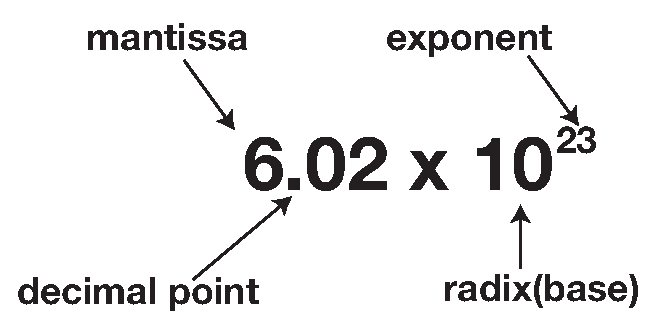
\includegraphics[keepaspectratio=true,width=0.3\linewidth]{figs/snfp.eps}
\caption{Scientific notation}
\label{fig:ex1}
\end{figure}

가수(mantissa or significand)와 지수(exponent or characteristic) 그리고 기저(base)가 사용되며 이것을 2진법 과학적 표기법을 사용하여 컴퓨터 1word에 저장시킨다. 32bit의 유동소수점(floating point)의 표현은 Figure~\ref{fig:ex2}와 같다.

\begin{figure}[!hbpt]
\centering
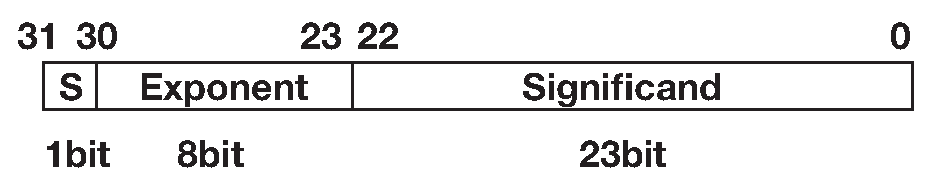
\includegraphics[keepaspectratio=true,width=0.6\linewidth]{figs/snfp2.eps}
\caption{32bit floating point}
\label{fig:ex2}
\end{figure}

\textbf{IEEE 754 Standard}\\

\begin{equation}
FPnumber = (-1)^{S}\cdot (1+Significand)\cdot 2^{Exponent}
\end{equation}

\begin{equation}
FPnumber = (-1)^{S}\cdot (1+Significand)\cdot 2^{Exponent-Bias}
\end{equation}
